\section{Thí nghiệm: đọc kết quả mà không phóng đại}
\label{sec:experiments}

\subsection{Ba câu hỏi thực nghiệm}

Paper đánh giá D-Tracker bằng ba câu hỏi:
\begin{description}[leftmargin=1.8em,style=nextline]
  \item[Q1 --- Accuracy.] Dự báo tương lai chính xác đến đâu, so với các phương pháp mạnh?
  \item[Q2 --- Scalability.] Thời gian chạy thay đổi thế nào khi stream dài hơn?
  \item[Q3 --- Effectiveness.] Mô hình có tách được trend, mùa vụ và lan truyền theo cách đọc được không?
\end{description}
Đừng gộp ba câu hỏi thành một. Một mô hình có thể thắng MAE nhưng không cho ta hiểu diffusion; một
hình diffusion đẹp không chứng minh dự báo tốt. Toàn bộ phần này nên đọc như ba lát cắt riêng,
cùng một mô hình.

\subsection{Dữ liệu}

Paper dùng năm stream GoogleTrends và một stream COVID-19. Bảng~\ref{tab:datasets} lấy trực tiếp
paper Table~4; kích thước ghi theo thứ tự (thời gian, từ khóa, địa điểm).

\begin{table}[htbp]
  \centering
  \small
  \caption{Sáu dataset trong paper (paper Table~4). Tên từ khóa được giữ nguyên như paper.}
  \label{tab:datasets}
  \begin{tabular}{@{}cl>{\raggedright\arraybackslash}p{5.6cm}c@{}}
    \toprule
    ID & Dataset & Từ khóa & Shape \\
    \midrule
    1 & Device & Apple Watch, Fitbit, Galaxy, Google Pixel, Macbook, Xperia, iPad, iPhone & $(676,8,50)$ \\
    2 & Pythonlib & matplotlib, numpy, pandas, pytorch, scipy, sklearn, tensorflow & $(676,7,50)$ \\
    3 & VoD & Apple TV, DAZN, HBO, Prime Video, hulu, netflix, youtube & $(676,7,50)$ \\
    4 & Chatapp & facebook, instagram, slack, snapchat, tiktok, twitter, viber, whatsapp & $(676,8,50)$ \\
    5 & Language & CSS, HTML, Java, JavaScript, PHP, Ruby, SQL, python, swift & $(676,9,50)$ \\
    6 & Covid-19 & new infected, new deceased & $(990,2,50)$ \\
    \bottomrule
  \end{tabular}
\end{table}

GoogleTrends là dữ liệu theo tuần, 2010--2022. Covid-19 là dữ liệu theo ngày, tháng 1/2020 đến
tháng 9/2022. Tất cả được chuẩn hóa min--max về $[0,1]$. Có một điểm không khớp nhỏ trong paper:
phần văn xuôi nói 48 quốc gia, còn paper Table~4 dùng 50 địa điểm. Tài liệu giữ cả hai và không tự
``sửa'' số nào.

\subsection{Thiết lập dự báo}

Với GoogleTrends, cửa sổ hiện tại dài $L_c=104$ tuần (hai năm). Tầm dự báo
$L_f\in\{13,26,39\}$ tuần, tương ứng 3, 6, 9 tháng. Với Covid-19, $L_c=56$ ngày (tám tuần) và
$L_f\in\{7,14,21\}$ ngày, được paper diễn giải là 1, 2, 3 tuần trong phần kết quả. Các baseline
gồm DISMO, FluxCube, PatchTST, Autoformer, DeepAR, LaST và CoST. Chi tiết huấn luyện và tìm
hyperparameter nằm ở Appendix~B.1; D-Tracker không huấn luyện lại từ đầu trên toàn bộ lịch sử ở
mỗi bước mà cập nhật theo cửa sổ.

\subsection{MAE và RMSE: đọc đúng chiều}

Với $n$ dự báo, gọi $y_i$ là giá trị thật và $\hat y_i$ là dự báo:
\[
  \mathrm{MAE}=\frac1n\sum_{i=1}^n|y_i-\hat y_i|,
  \qquad
  \mathrm{RMSE}=\sqrt{\frac1n\sum_{i=1}^n(y_i-\hat y_i)^2}.
\]
Cả hai đều \textbf{nhỏ hơn là tốt hơn}. MAE đo sai số trung bình; RMSE phạt sai số lớn mạnh hơn.
Ví dụ minh họa: hai dự báo sai lệch $-0.04$ và $+0.08$ có MAE $=0.06$ và
RMSE $=\sqrt{(0.0016+0.0064)/2}\approx0.063$. Đây là ví dụ tự tạo để hiểu metric, không phải kết quả
paper.

\begin{commonmistake}
Không được so sánh trực tiếp một MAE $0.84$ trong paper Table~3 với một giá trị thô $0.84$ của dữ liệu
chưa chuẩn hóa. Tiêu đề bảng ghi các giá trị theo đơn vị $\times10^{-2}$; tài liệu giữ nguyên số in
trong bảng và không tự đổi đơn vị. Khi báo cáo lại, phải nói rõ đơn vị.
\end{commonmistake}

\subsection{Kết quả Q1: độ chính xác}

Bảng~\ref{tab:dtracker-mae} chỉ chép các dòng D-Tracker từ paper Table~3, không chép baseline.
Paper kết luận D-Tracker có MAE tốt nhất trên \emph{tất cả} dataset và giảm RMSE đáng kể, nhưng
cũng thừa nhận một số RMSE tương đương vì RMSE nhạy với lỗi lớn. Đây là hai phát biểu cần giữ cùng
nhau.

\begin{table}[htbp]
  \centering
  \scriptsize
  \caption{MAE và RMSE của D-Tracker trong paper Table~3, giữ đúng các giá trị in trong paper
  (đơn vị bảng: $\times10^{-2}$). Cột 1/2/3 là ba horizon $L_f$ theo thứ tự trong tên dataset.}
  \label{tab:dtracker-mae}
  \begin{tabular}{@{}lccccccc@{}}
    \toprule
    & & \multicolumn{3}{c}{MAE} & \multicolumn{3}{c}{RMSE} \\
    \cmidrule(lr){3-5}\cmidrule(lr){6-8}
    Dataset & $L_f$ & 1 & 2 & 3 & 1 & 2 & 3 \\
    \midrule
    Device & 13/26/39 & 0.84 & 0.90 & 0.97 & 1.82 & 1.95 & 2.18 \\
    Pythonlib & 13/26/39 & 0.27 & 0.32 & 0.37 & 1.42 & 1.54 & 1.78 \\
    VoD & 13/26/39 & 0.53 & 0.59 & 0.63 & 1.58 & 1.83 & 2.02 \\
    Chatapp & 13/26/39 & 0.28 & 0.34 & 0.41 & 0.83 & 1.01 & 1.24 \\
    Language & 13/26/39 & 0.31 & 0.35 & 0.40 & 0.97 & 1.14 & 1.32 \\
    Covid-19 & 7/14/21 & 0.47 & 0.70 & 0.98 & 1.40 & 2.42 & 3.65 \\
    \bottomrule
  \end{tabular}
\end{table}

Hai con số được nhắc ở bullet cuối §1 là ``cải thiện tới 57\%'' và ``nhanh tới 8.0 lần''.
Paper không nêu mẫu số của 57\% ngay tại câu đó, nên tài liệu chỉ được viết ``paper báo cáo tối đa
57\%'', không tự tính lại hay gán cho một metric cụ thể. Tương tự, 8.0 lần là kết quả trên cấu hình
phần cứng của paper, không phải hằng số cho mọi máy.

\subsection{Ablation: thành phần nào đóng góp?}

\begin{figure}[htbp]
  \centering
  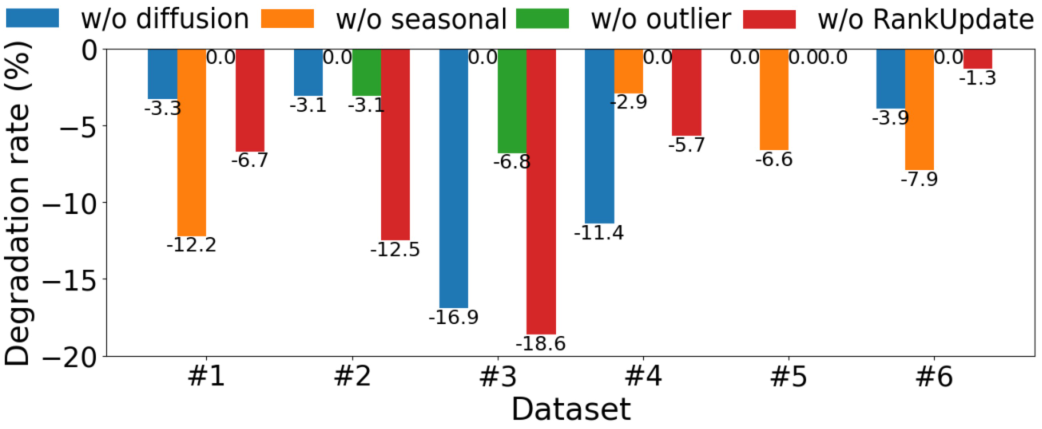
\includegraphics[width=0.95\linewidth]{figures/drop_rate.png}
  \caption{Ablation study của paper. Cột càng cao thể hiện mức giảm chất lượng khi bỏ một thành
  phần. Nguồn: Higashiguchi et al. (2025), arXiv:2505.00242v1, Figure~3; hình của tác giả,
  CC BY 4.0.}
  \label{fig:ablation}
\end{figure}

Hình~\ref{fig:ablation} bỏ lần lượt diffusion, seasonal, outlier và RankUpdate. Các degradation rate
được đo ở horizon 26 tuần (GoogleTrends) hoặc 14 ngày (Covid-19). Paper báo cáo:
\begin{itemize}
  \item seasonal cải thiện rõ ở các dataset có mùa vụ mạnh như Device, Language và Covid-19;
  \item diffusion cải thiện rõ ở VoD và Chatapp;
  \item outlier giúp ở một số dataset nhờ lọc các thay đổi đột ngột;
  \item RankUpdate giúp mô hình thích nghi khi số chiều tối ưu thay đổi.
\end{itemize}
Điều quan trọng không kém là các ngoại lệ. Ở Language, diffusion không cải thiện; paper diễn giải
rằng có thể có rất ít lan truyền giữa các quốc gia cho các ngôn ngữ lập trình. Ở dataset không có
nhiều mùa vụ/outlier, hai thành phần này có thể không giúp. Một mô hình ``thắng trung bình'' không
có nghĩa mọi module đều hữu ích ở mọi nơi.

\subsection{Q2: scalability}

\begin{figure}[htbp]
  \centering
  \begin{subfigure}[t]{0.49\linewidth}
    \centering
    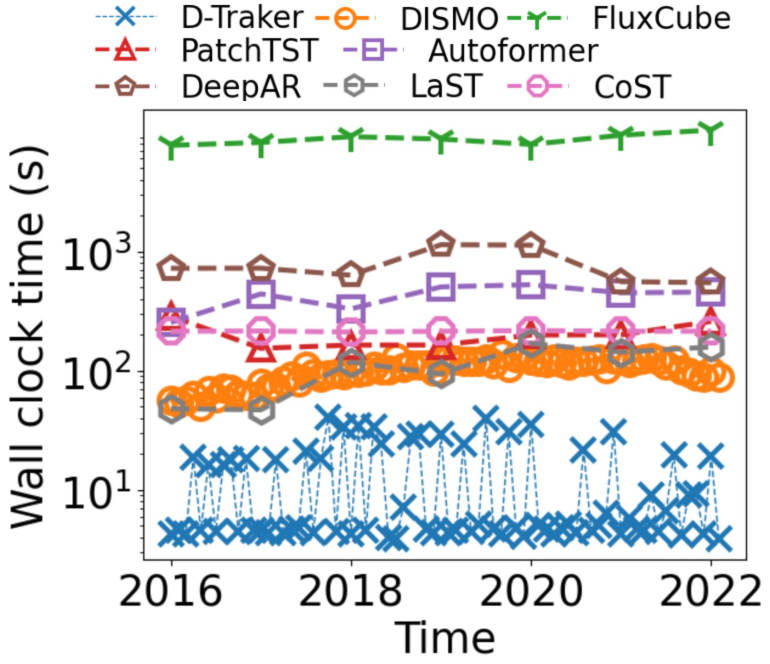
\includegraphics[width=\linewidth]{figures/scalability.png}
    \caption{Thời gian theo chiều dài stream.}
  \end{subfigure}\hfill
  \begin{subfigure}[t]{0.49\linewidth}
    \centering
    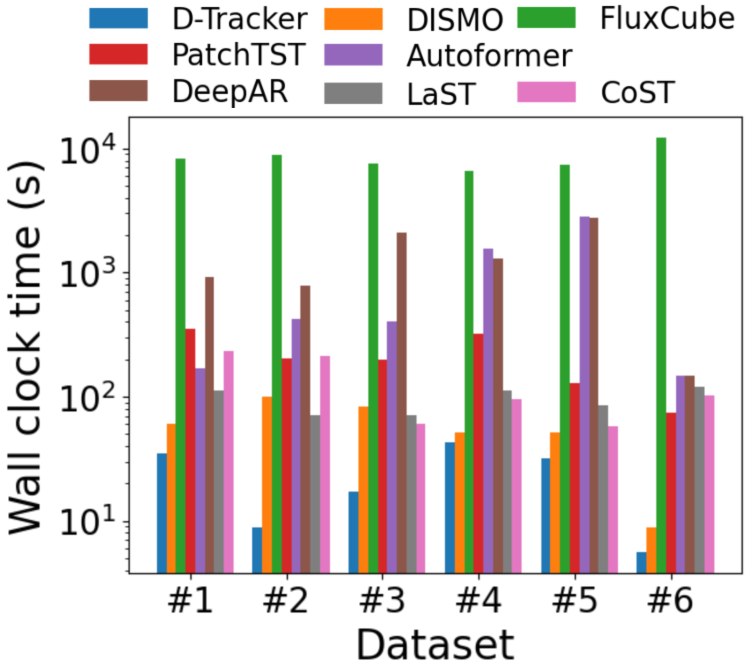
\includegraphics[width=\linewidth]{figures/avgtime.png}
    \caption{Thời gian trung bình trên toàn stream.}
  \end{subfigure}
  \caption{ Scalability của D-Tracker trên Pythonlib. Nguồn: Higashiguchi et al. (2025),
  arXiv:2505.00242v1, Figure~4; hình của tác giả, CC BY 4.0.}
  \label{fig:scalability}
\end{figure}

Ở Hình~\ref{fig:scalability}, thời gian xử lý của D-Tracker gần như phẳng khi stream dài thêm, trong
khi các baseline có xu hướng tăng. Các ``spike'' nhỏ là lúc RankUpdate chạy ModelEstimation nhiều
lần. Đây là bằng chứng cho tuyên bố ``thời gian không phụ thuộc chiều dài stream'', nhưng không
phải bằng chứng rằng mọi phép tính là hằng số: chi phí vẫn phụ thuộc số từ khóa, địa điểm, rank và
số lần cập nhật cấu trúc.

\subsection{Q3: mô hình có diễn giải được không?}

\begin{figure}[htbp]
  \centering
  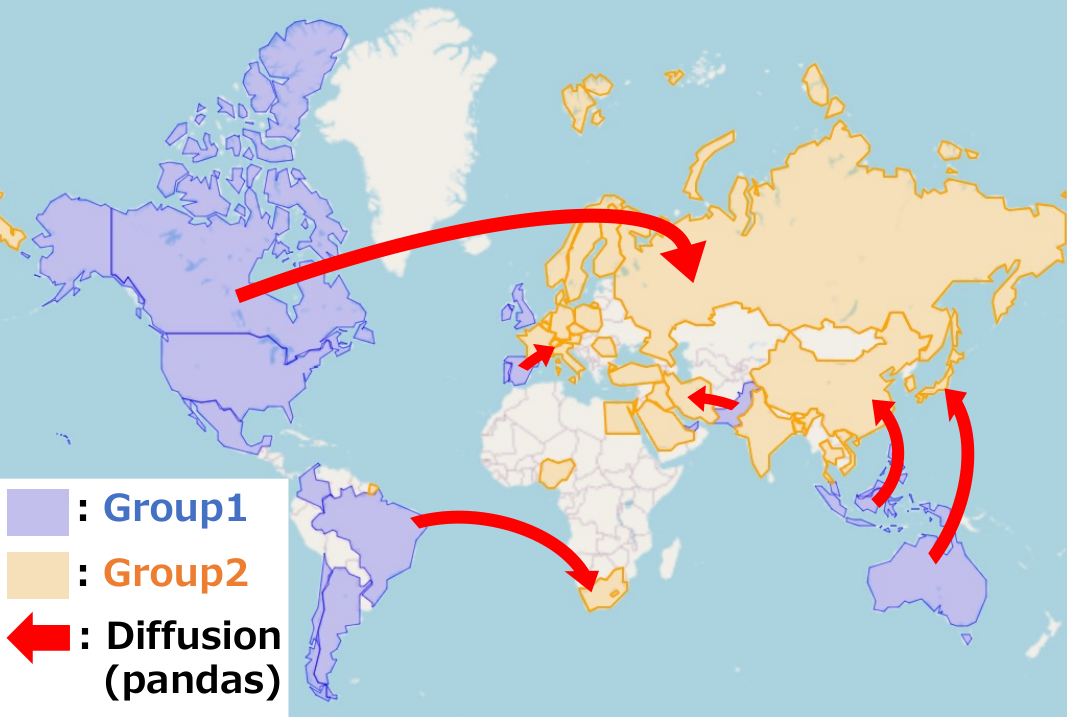
\includegraphics[width=0.78\linewidth]{figures/diff_2014.png}
  \caption{Một phần kết quả mô hình hóa Pythonlib 2013--2015: pattern lan truyền được hệ
  reaction--diffusion gán cho ``pandas''. Nguồn: Higashiguchi et al. (2025), arXiv:2505.00242v1,
  Figure~5; hình của tác giả, CC BY 4.0.}
  \label{fig:diffusion-example}
\end{figure}

Paper đọc Ví dụ~\ref{fig:diffusion-example} như sau: dynamics liên quan đến ``pandas'' lan từ nhóm
địa điểm gồm Bắc Mỹ và Australia sang nhóm gồm các nước châu Á, chủ yếu Trung Quốc. Đây là một
\emph{diễn giải có cấu trúc}: hệ số từ khóa nói ``pandas'', hệ số địa điểm chia nhóm, và tham số
diffusion nói hướng. Nó không chứng minh quan hệ nhân quả; để kiểm chứng cần dữ liệu ngoài mô hình
hoặc thiết kế thí nghiệm phù hợp.

\subsection{Điều paper không chứng minh}

Paper không báo cáo khoảng tin cậy, kiểm định thống kê hay xác suất dự báo. Nó cũng không chứng minh
D-Tracker luôn thắng mọi baseline trên mọi horizon; kết luận là trên sáu stream và các thiết lập đã
nêu. Vì vậy, câu đúng là ``trong thí nghiệm này, D-Tracker đạt MAE tốt nhất và thời gian chạy thấp
hơn'', không phải ``D-Tracker là phương pháp tốt nhất cho mọi dữ liệu chuỗi thời gian''.

\begin{keypoint}
Ba kết quả nên nhớ: (1) D-Tracker đứng đầu MAE trên sáu dataset theo paper Table~3; (2) thời gian mỗi
bước không tăng theo chiều dài stream nhờ cửa sổ cố định, với các spike khi đổi rank; (3) mô hình
cho ra các nhóm và hướng diffusion đọc được, nhưng đó là diễn giải theo giả định, không phải nhân
quả đã kiểm chứng.
\end{keypoint}

\begin{selfcheck}
\begin{enumerate}
  \item Vì sao MAE và RMSE có thể xếp hạng hai mô hình khác nhau?
  \item Trong ablation, vì sao bỏ diffusion không làm giảm chất lượng ở Language?
  \item Giải thích vì sao ``thời gian không phụ thuộc chiều dài stream'' không đồng nghĩa $O(1)$.
  \item Nêu một kết luận \emph{không} thể rút ra từ Figure~\ref{fig:diffusion-example}.
\end{enumerate}
\end{selfcheck}
